%!TEX root = ../thesis.tex
%*******************************************************************************
%****************************** Second Chapter *********************************
%*******************************************************************************

\chapter{Background}
\label{chapter2}

\ifpdf
    \graphicspath{{Chapter2/Figs/Raster/}{Chapter2/Figs/PDF/}{Chapter2/Figs/}}
\else
    \graphicspath{{Chapter2/Figs/Vector/}{Chapter2/Figs/}}
\fi

%********************************** %First Section  **************************************
\section{Lattice models}
\label{sec:lattice-models}

\subsection{Historical introduction}
\label{subsec:latt-hist}
I think starting from the magnetism point of view might be the best way to go, slowly lead into the field of condensed matter theory and lattice models. 

\subsection{The Schr{\"o}dinger equation and the Feynman path integral}
\label{subsec:latt-qm}
The wavefunction
\begin{equation}
	\Psi\left(r_{1}, \ldots, r_{N}\right)
\end{equation}
the Schr\" odinger equation
\begin{equation}
	i \frac{\partial \psi(\boldsymbol{r}, t)}{\partial t}= \hat{H} \psi(\textbf{r}, t)
\end{equation}
for a single particle in an external potential $\hat{V}(\boldsymbol{r})$ the Hamiltonian is 
\begin{equation}
	\hat H \phi(\boldsymbol{r})=-\frac{1}{2} \nabla^{2} \phi(\boldsymbol{r})+\hat{V}(\boldsymbol{r}) \phi(\boldsymbol{r}).
\end{equation}
Alternatively to the Schr\" odinger equation one can use an integral Green's function representation to express the wavefunction $\psi$ at some future time $t_2$ given initial condition $\psi(\boldsymbol{r}, t_1)$ as
\begin{equation}
	\psi\left(\boldsymbol{r}_{2}, t_{2}\right)=\int  \mathcal{K}\left(\boldsymbol{r}_{2}, t_{2} ; \boldsymbol{r}_{1}, t_{1}\right) \psi\left(\boldsymbol{r}_{1}, t_{1}\right) \mathrm{d} \boldsymbol{r}_{1}.
\end{equation}
The solution to  equation
\begin{equation}
	\left(i \frac{\partial}{\partial t_{2}}-H_{\boldsymbol{r}_{2}}\right) \mathcal{K}\left(\boldsymbol{r}_{2}, t_{2} ; \boldsymbol{r}_{1}, t_{1}\right)=i \delta\left(\boldsymbol{r}_{1}-\boldsymbol{r}_{2}\right) \delta\left(t_{1}-t_{2}\right)
\end{equation}
and the \textit{propagator} $\mathcal{K}\left(\boldsymbol{r}_{2}, t_{2} ; \boldsymbol{r}_{1}, t_{1}\right)$ is expressed using the Feynman path integral
\begin{equation}
	\label{eq:FPI}
	\mathcal{K}\left(\boldsymbol{r}_{2}, t_{2} ; \boldsymbol{r}_{1}, t_{1}\right)=\int_{\boldsymbol{r}\left(t_{1}\right)=r_{1} \atop \boldsymbol{r}\left(t_{2}\right)=r_{2}} \mathcal{D} \boldsymbol{r}(t) \exp \left(i \int_{t_{1}}^{t_{2}} \mathcal{L}(\boldsymbol{r}, \dot{\boldsymbol{r}}) d t\right),
\end{equation}
where $\mathcal{L}$ is the classical Lagrangian function of the system
\begin{equation}
	L(\boldsymbol{r}, \dot{\boldsymbol{r}})=\frac{1}{2} \dot{\boldsymbol{r}}^{2}-\hat V(\boldsymbol{r}),
\end{equation}
and the integral is over all paths that satisfy the endpoint conditions.

\subsection{Examples of lattice models}
\label{subsec:latt-examples}

\begin{equation}
	\hat{\sigma}^x_{i}=\left(\begin{array}{cc}0 & 1 \\ 1 & 0\end{array}\right)_{i} \quad \hat{\sigma}^y_{i}=\left(\begin{array}{cc}0 & -i \\ i & 0\end{array}\right)_{i} \quad \hat{\sigma}^z_{i}=\left(\begin{array}{cc}1 & 0 \\ 0 & -1\end{array}\right)_{i}
\end{equation}


\subsubsection{Transverse Field Ising model}
\begin{equation}
	\hat H_{\mathrm{Ising}}=-J \sum_{\langle i, j\rangle} \hat{\sigma}^z_{i} \hat{\sigma}^z_{j}-h \sum_{i} \sigma^x_{i}
\end{equation}

\subsubsection{Heisenberg model}
\begin{equation}
	\hat{H}_{\mathrm{Heisenberg}}=-\frac{1}{2} \sum_{j=1}^{N}
	\left[J_{x} \hat{\sigma}_{j}^{x} \hat{\sigma}_{j+1}^{x}+J_{y} \hat{\sigma}_{j}^{y} \sigma_{j+1}^{y}+J_{z} \hat{\sigma}_{j}^{z} \hat{\sigma}_{j+1}^{z}+h \hat{\sigma}_{j}^{z}
	\right]
\end{equation}

\subsubsection{Bose-Hubbard model}
\begin{equation}
	\hat{H}_{\mathrm{BH}}= -t \sum_{\langle i, j\rangle} \hat{b}_{i}^{\dagger} \hat{b}_{j}+\frac{U}{2} \sum_{i} \hat{n}_{i}\left(\hat{n}_{i}-1\right)-\mu \sum_{i} \hat{n}_{i}
\end{equation}


%********************************** %Second Section  *************************************

\newpage
\section[The Feynman-Kac formula]{Feynman-Kac: connecting Quantum Mechanics and Stochastic Processes}
\label{subsec:FK}

\subsection{Stochastic processes}
\label{subsec:fk-stoch}
Introduce minimal necessary basics to understand the following section/discussions. This includes
\begin{itemize}
	\item Random variables
	\item Markov chains
	\item Transition matrices
	\item Brownian walk, measures on the Brownian walk. 
\end{itemize}

\begin{figure}[h]
	\centering
	\includegraphics[width=0.7\linewidth]{example-image-golden}
\end{figure}

\subsection{Feynman-Kac formula}
\label{subsec:fk-fk}
The Feynman path integral formulation~\eqref{eq:FPI} was extensively used by physicists for decades, even in the absence of a formal mathematical formulation which is hard to define because of the difficulties with defining an appropriate measure on the path space. Kac~\cite{kac1949distributions} provided a rigorous formulation of the \textit{real-valued} case of the Feynman path integral, and the resulting \emph{Feynman-Kac} formula provides a bridge between \emph{parabolic} partial differential equations and stochastic processes.

To illustrate the Feynman-Kac formula let us consider a single particle with Hamiltonian
\begin{equation}
	\hat{H} = -\frac{\mathrm{d}^2~~}{\mathrm{d}x^2} + V(x)
\end{equation}
and the Schr\" odinger equation in \textit{imaginary time}, which is of the elliptic type, 
\begin{equation}
	\partial_t | \psi_t \rangle = - \hat{H} | \psi_t \rangle.
\end{equation}
Its formal solution, the time propagation of an initial wave function $|\phi_0\rangle$ at $t=0$, is written as
\begin{equation}
	\left| \psi_{t} \right\rangle = e^{-\hat{H} t}\left|\psi_{0}\right\rangle. 
\end{equation}
From the spectral decomposition of the operator $e^{-\hat{H} t}$ in terms of eigenstates $|\phi_n\rangle$ and eigen-energies $E_n$ of the Hamiltonian $\hat{H}$
\begin{equation}
	e^{-\hat{H} t}=\sum_{n} e^{-E_{n} t}|\phi_n\rangle\langle\phi_n|, 
\end{equation}
it follows that the term corresponding to the ground state of the system $|\phi_0\rangle$ decays the slowest. Thus starting in some initial state and propagating for a long imaginary time $it$ leads into the ground state with the decay rate giving the ground state energy as
\begin{equation}
	\lim_{t \rightarrow \infty} | \psi_t \rangle \propto e^{-E_0 t} | \phi_0 \rangle,
\end{equation} 
where $E_0$ is the ground state energy and $|\phi_0\rangle$ is the corresponding state. Kac noticed that the kinetic term of the Lagrangian in~\eqref{eq:FPI} could be interpreted as a measure on Brownian walks, and a solution to the imaginary time Schr\" odinger equation can be written as
\begin{equation}
	\psi(x, t)=\underset{X \sim \text { Brownian with } X_{t}=x}{\mathbb{E}}
	\left[\exp \left(-\int_{0}^{t}  V\left(X_{\tau}, \tau \right) \mathrm{d}\tau \right) \psi\left(X_{0}, 0\right)\right],
\end{equation}
where only the \textbf{endpoint} at time $t$ of the Brownian process fixed, whereas the starting point at time $t=0$ is not, $\psi (x, 0)$ encodes the initial condition into this representation. When there is no external potential $V(x) = 0$, the Schr\" odinger equation in imaginary time is the diffusion equation and the Feynman-Kac solution is simply
\begin{equation}
	\begin{aligned} 
		\psi(x, t) &= \underset{X \sim \text { Brownian with } X_{t}=x}{\mathbb{E}}\left[\psi\left(X_{0}, 0\right)\right] \\
		&=  
		\frac{1}{\sqrt{2 \pi t}} \int  e^{-\left(x-x^{\prime}\right)^{2} / 2 t} \psi_{0}\left(x^{\prime}\right) \mathrm{d} x^{\prime}
	\end{aligned}
\end{equation}
An illustration of the Feynman-Kac approach to the problem with no external potential $V(x)$ in 1D is depicted in figure~\ref{fig:fk_1d_example}
\begin{figure}[h]
	\centering
	\subfloat
	{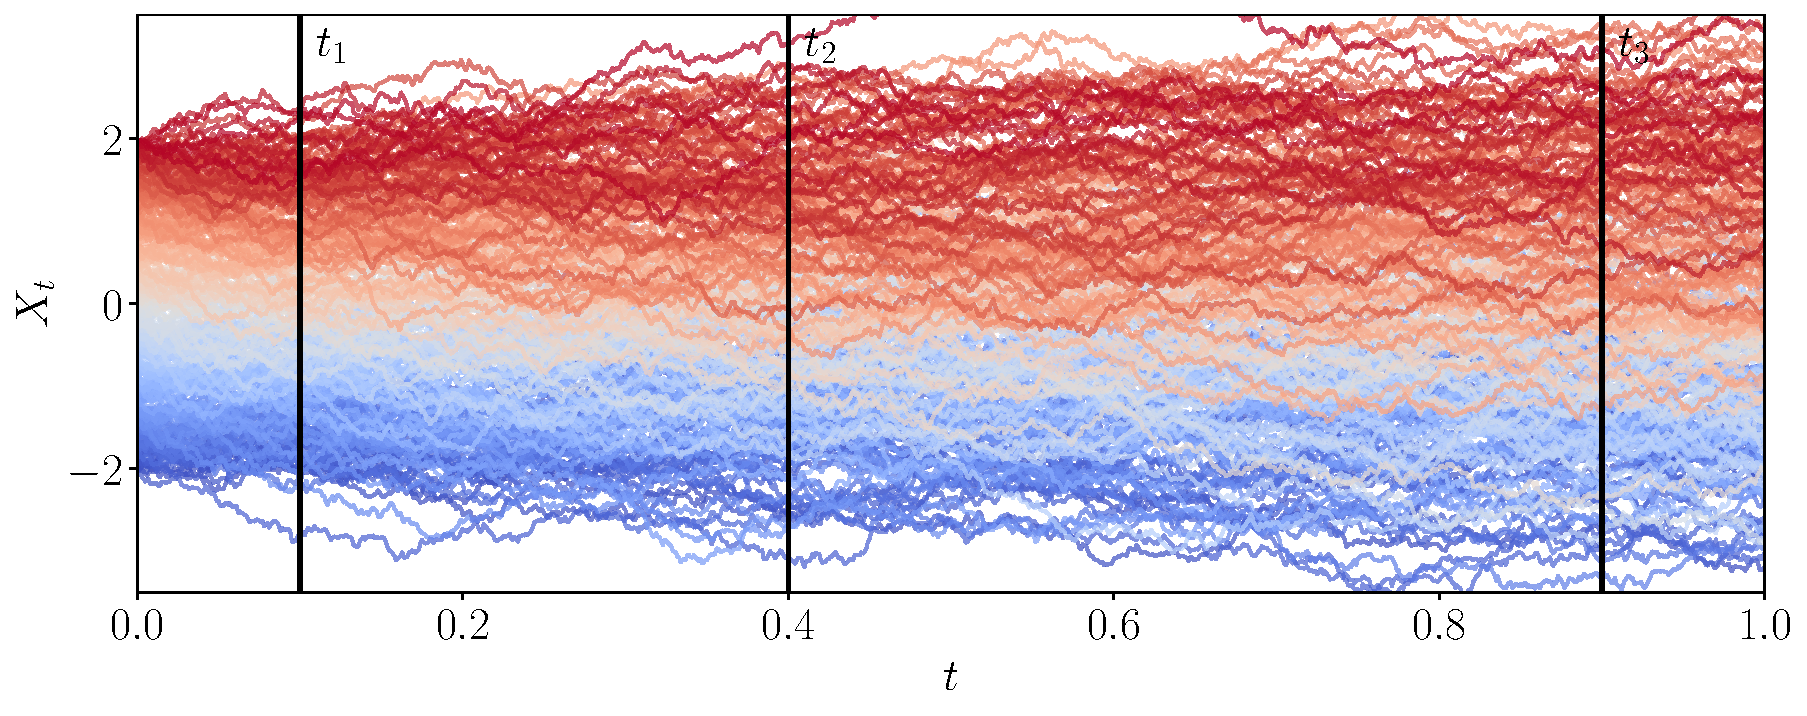
\includegraphics[width = \linewidth]{Chapter2/Figs/Raster/fkac_vs_fplanck_top.pdf}} \\
	\subfloat
	{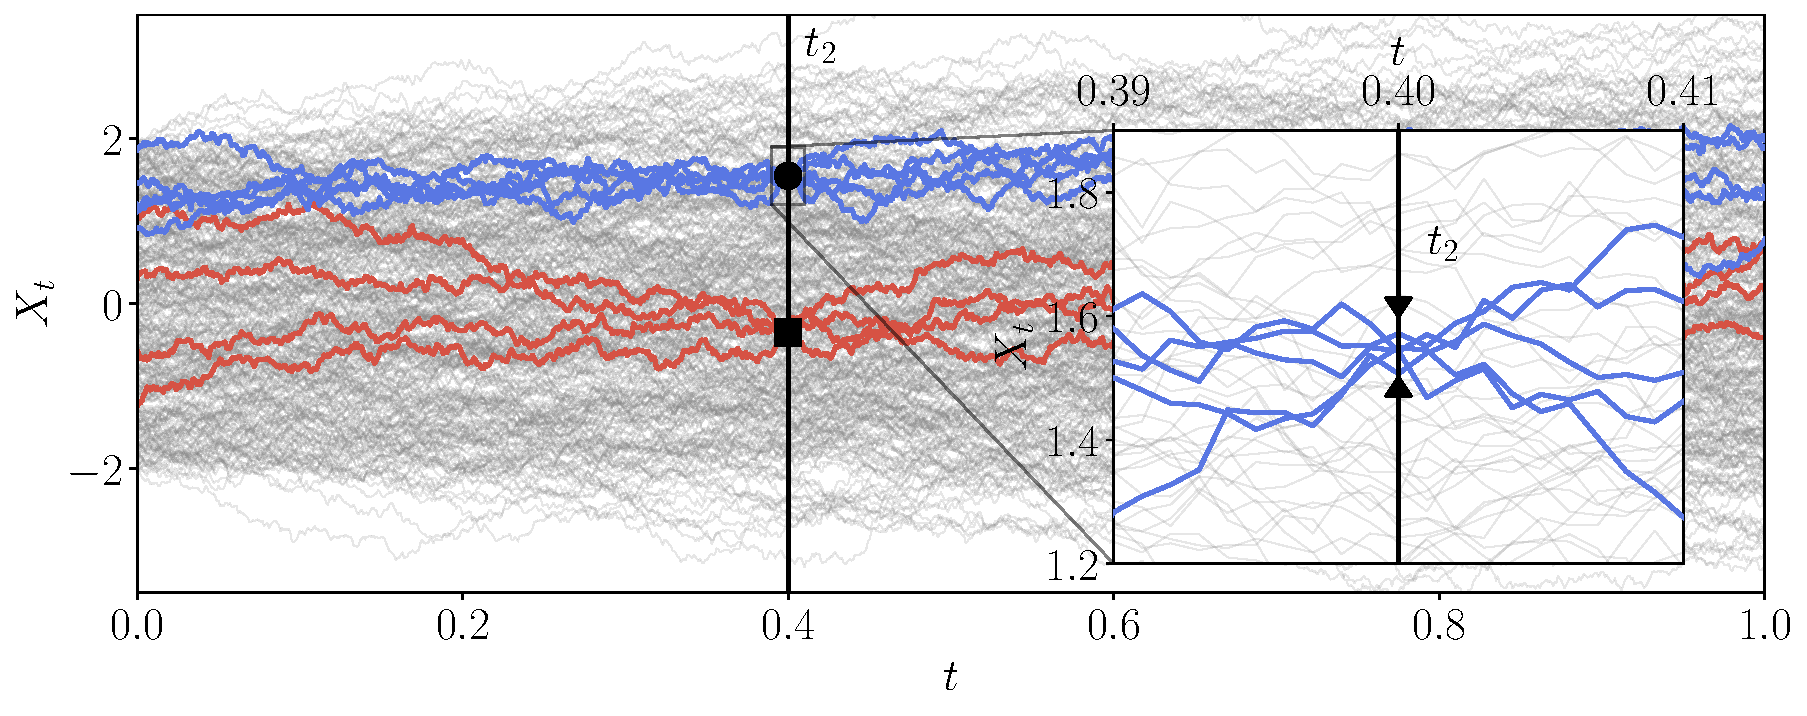
\includegraphics[width = \linewidth]{Chapter2/Figs/Raster/fkac_vs_fplanck_mid1.pdf}} \\
	\subfloat
	{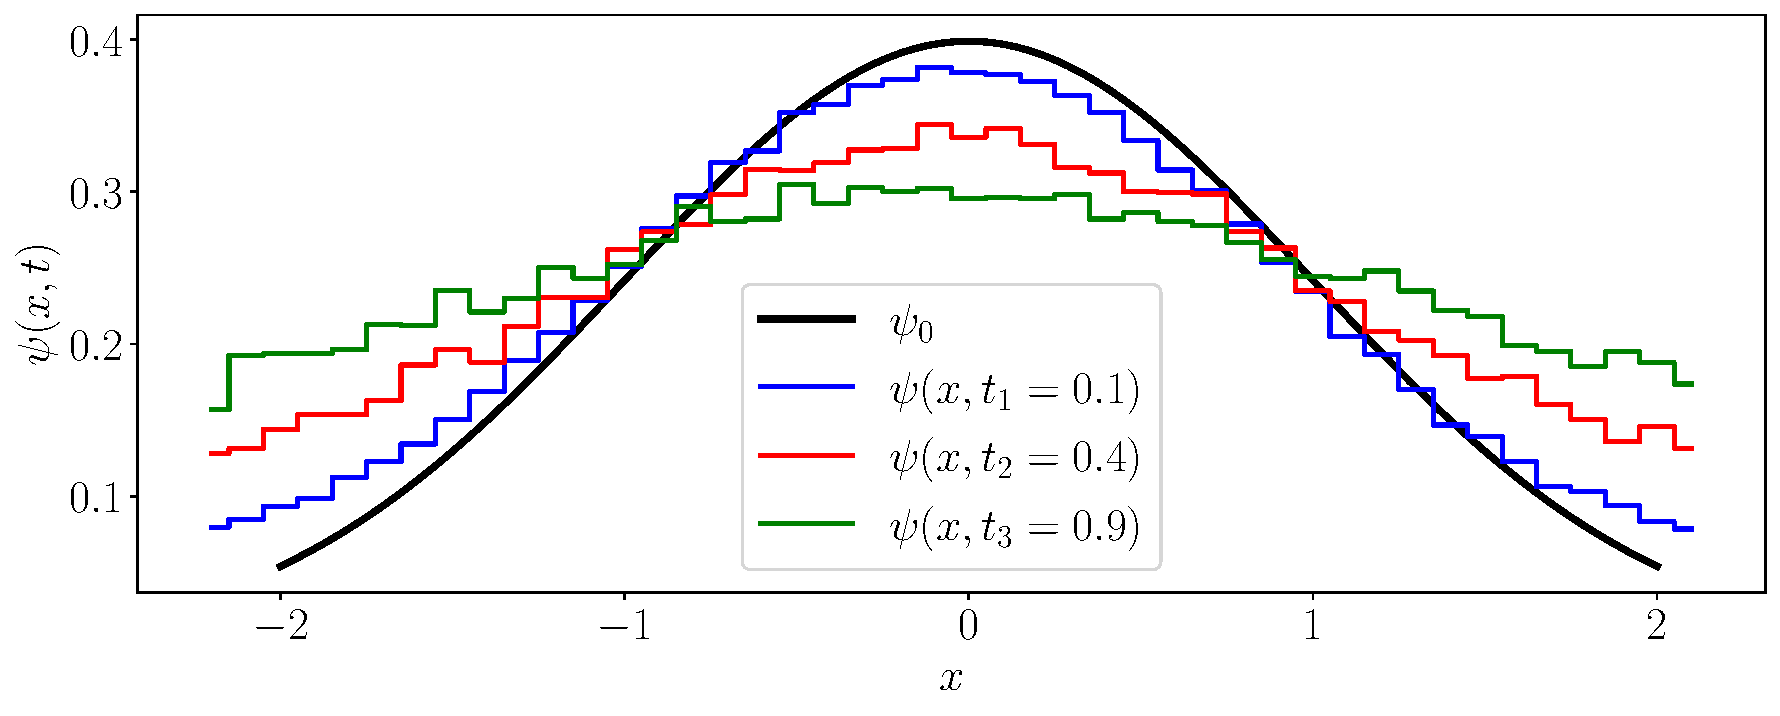
\includegraphics[width = \linewidth]{Chapter2/Figs/Raster/fkac_vs_fplanck_bottom.pdf}}
	
	\caption[Feynman-Kac for a 1D free particle]{\textbf{Feynman-Kac for a 1D free particle.} \textbf{top:} $N=400$ Brownian walks starting from different $x_0$, the color signifies initial position. In order to evaluate $\psi$ between $x-\frac{\delta x}{2}$ and $x+\frac{\delta x}{2}$ at some time $t$ we must first find Brownian paths that end there. \textbf{middle:} The paths that pass through at $x \in (1.5, 1.6)$ (blue) and through $x \in (-0.4,-0.3)$ (red) are colored, others are left in grey. \textbf{bottom:} Time evolution of the initial condition $\psi_{0} = \frac{1}{\sqrt{2 \pi}} e^{-\frac{1}{2} x^{2}}$, by estimating ${\mathbb{E}}\left[\psi\left(X_{0}, 0\right)\right]$ from the filtered paths at each timestep.}
	\label{fig:fk_1d_example}
\end{figure}


\subsection{Stoquastic Hamiltonians and Lattice-model representations}
\label{subsec:fk-latt}
\begin{figure}[h]
	\centering
	\includegraphics[width=0.3\textwidth]{example-grid-100x100pt}
\end{figure}

general Stochquastic hamiltonian -> Feynman kac for general process

\subsubsection{Quantum Ising model}
\subsubsection{Heisenberg model}
\subsubsection{Bose-Hubbard model}


%********************************** % ??? Section  *************************************
\newpage
\section{Quantum Monte Carlo}
\label{sec:qmc}

Nekje povej, kaksen complexity imajo QMC problemi za fermione in bozone. 

\subsection{Overview}
\label{subsec:qmc-overview}

%********************************** % ??? Section  *************************************
\newpage
\section{Machine Learning}
\label{sec:ml}

\subsection{Convolutional Neural Networks}
\label{subsec:ml-cnn}

\subsection{Overview of ML approaches to the Quantum many-body problem}
\label{subsec:ml-overview}
